


\documentclass[]{article}
%
% If IEEEtran.cls has not been installed into the LaTeX system files,
% manually specify the path to it like:
% \documentclass[journal]{../sty/IEEEtran}

\usepackage{amsmath, amsthm, amssymb,bm,datetime}
\usepackage{graphicx,color,subfigure}
%\usepackage{hyperref}
\usepackage{epstopdf}
\usepackage{booktabs}
\usepackage{cases}
\usepackage{cite}
\usepackage[margin=0.75in]{geometry}
\usepackage{authblk}




\newcommand{\re}{\mathbb R}
\newcommand{\Ex}[2]{\mathcal{E}^{#2}[#1]}
%\newcommand{\log}{\text{log}[#1]}
\newcommand{\Tr}{\mathbf{Tr}}
\newcommand{\etal}{\textit{et al. }}

\newcommand{\eq}[1]{Eq.~(\ref{#1})}
\newcommand{\Fig}[1]{Fig.~\ref{#1}}

\renewcommand{\v}[1]{\ensuremath{\mathbf{#1}}}
\newcommand{\vo}[1]{\ensuremath{\boldsymbol{#1}}}
\newcommand{\pderiv}[2]{\frac{\partial #1}{\partial #2}}

\newcommand{\eps}{\boldsymbol{\epsilon}}
\newcommand{\Nu}{\boldsymbol{\nu}}
\newcommand{\Ps}{\boldsymbol{\Psi}}
\newcommand{\xii}{\boldsymbol{\xi}}
\newcommand{\Al}{\boldsymbol{\alpha}}
\newcommand{\x}{\mathbf{x}}
\newcommand{\s}{\mathbf{s}}
\newcommand{\C}{\mathbf{C}}
\newcommand{\uu}{\mathbf{u}}
\newcommand{\z}{\mathbf{z}}
\newcommand{\q}{\mathbf{q}}
\newcommand{\A}{\mathbf{A}}
\newcommand{\B}{\mathbf{B}}
\newcommand{\K}{\mathbf{K}}
\newcommand{\f}{\mathbf{f}}
\newcommand{\hc}{\mathbf{H}}
\newcommand{\R}{\mathbf{R}}
\newcommand{\G}{\mathbf{G}}
\newcommand{\y}{\mathbf{y}}
\newcommand{\Y}{\mathbf{Y}}
\newcommand{\teta}{\boldsymbol{\theta}}
\newcommand{\Teta}{\boldsymbol{\Theta}}
\newcommand{\pe}{\hat{\mathbf{p}}}
\newcommand{\pl}{\mathbf{p}^{(l)}}
\newcommand{\pt}{\mathbf{p}^\text{true}}

\newcommand{\kk}{\mathcal{K}}
\newcommand{\p}{\mathcal{P}}
%\DeclareMathOperator{\Exp}{E}
\newcommand{\V}{{\mathpzc{V}}}
\newcommand{\E}{{\mathpzc{E}}}

\newcommand{\bs}{b}
\newcommand{\bv}{\mathbf{b}}
\newcommand{\bme}{z}
\newcommand{\bvm}{\tilde{\bv}}
\newcommand{\xg}{x^G}
\newcommand{\yg}{y^G}
\newcommand{\kbf}{\mathbf{k}}
\newcommand{\mbf}{\mathbf{m}}
\newcommand{\Pbf}{\mathbf{P}}
\newcommand{\Rbf}{\mathbf{R}}
\newcommand{\Vbf}{\mathbf{V}}
\newcommand{\xbf}{\mathbf{x}}
\newcommand{\Xbf}{\mathbf{X}}
\newcommand{\Ybf}{\mathbf{Y}}
\newcommand{\zbf}{\mathbf{z}}
\newcommand{\Zbf}{\mathbf{Z}}
\newcommand{\mubf}{\boldsymbol{\mu}}
\newcommand{\nubf}{\boldsymbol{\nu}}
\newcommand{\im}{\mathrm{i}}
\newcommand{\Gammabf}{\mathbf{\Gamma}}
\newcommand{\Cbf}{\mathbf{C}}
\newcommand{\Sigmabf}{\boldsymbol{\Sigma}}
\newcommand{\zcond}{\mathbf{z}\mid\mu}
\newcommand{\zcondbf}{\mathbf{z}\mid\boldsymbol{\mu}}
\newcommand{\signalG}{\mathcal{G}\paren{\mu,\mathbf{k}}}
\newcommand{\Gscript}{\mathcal{G}}
\newcommand{\sumnn}{\sum\limits_{n=1}^N}

\newcommand{\arr}[2]{\begin{array}{#1} #2 \end{array}}
\newcommand{\lbrcarray}[2]{\left\{\arr{#1}{#2}\right.}
\newcommand{\rbrcarray}[2]{\left.\arr{#1}{#2}\right\}}
\newcommand{\argminx}{\arg\min_X}
\newcommand{\Nscript}{\mathcal{N}}

%\DeclareMathOperator{\diag}{diag} 
\newcommand{\brkarray}[2]{\bracket{\arr{#1}{#2}}}



\begin{document}
\title{Synthetic MR : Optimal Experimental Design
%{\color{red}
% - other titles
% - Accelerated MR Thermometry Reconstruction in the Presence of Signal Model Uncertainties
% - Model-based Acceleration of MR Thermal Imaging Reconstruction in the Presence of Uncertainties
%}
}
%
%
% author names and IEEE memberships
% note positions of commas and nonbreaking spaces ( ~ ) LaTeX will not break
% a structure at a ~ so this keeps an author's name from being broken across
% two lines.
% use \thanks{} to gain access to the first footnote area
% a separate \thanks must be used for each paragraph as LaTeX2e's \thanks
% was not built to handle multiple paragraphs
%

\author[1]{Reza~Madankan*}
%\author[1]{Wolfgang~Stefan}
%\author[1]{Samuel Fahrenholtz}
%\author[1]{Christopher MacLellan}
%\author[1]{John~Hazle}
%\author[1]{Jason Stafford}
%\author[2]{Jeffrey S.~Weinberg, Ganesh~Rao}
%\author[1]{David~Fuentes}

\affil[1]{Department of Imaging Physics, University of Texas MD Anderson Cancer Center, e-mail: rmadankan@mdanderson.org}
%\affil[2]{Department of Neurosurgery, University of Texas MD Anderson Cancer Center}


% make the title area
\date{}
\maketitle{}

% As a general rule, do not put math, special symbols or citations
% in the abstract or keywords.
%\begin{abstract}
%TBD ...
%\end{abstract}
%\subsection*{keywords}
%MRI, thermal ablation, Arrhenius dose, inverse problems, mutual information, sensor management, quantification and estimation, Pennes bioheat model.






% For peer review papers, you can put extra information on the cover
% page as needed:
% \ifCLASSOPTIONpeerreview
% \begin{center} \bfseries EDICS Category: 3-BBND \end{center}
% \fi
%
% For peerreview papers, this IEEEtran command inserts a page break and
% creates the second title. It will be ignored for other modes.


\section*{Introduction}


\section*{Problem Statement}\label{sec:prob_statement}
Consider a magnetization signal $M_{TD}$ that is defined as

\begin{equation}\label{mtd}
M_{TD}(\kk,\p,\x)=\left(M_0(\x)\frac{1-(1-\cos \theta)e^{-\frac{T_D}{T_1(\x)}}-\cos \theta e^{-\frac{T_D}{T_1(\x)}}}{1-\cos \theta e^{-\frac{T_R}{T_1(\x)}}cos \alpha}\right) e^{-\frac{T_E}{T_2(\x)}}
\end{equation}
where, $M_0$ is the unsaturated magnetization, $\theta$ represents the flip angle, and $T_R$ and $T_E$ denote repetition time and echo time, respectively. Parameters $T_1$ and $T_2$ represents relaxation times, and $\alpha$ is the excitation pulse. Note that the unsaturated magnetization $M_0$, along with relaxation times $T_1$ and $T_2$, are a function of spatial coordination $\x$. As well, excitation pulse $\alpha$ is a function of flip angle in general, i.e. $\alpha=\alpha(\theta)$.

In practice, the MRI observations are Fourier transform of $M_{TD}$, usually polluted with a white noise $\nu$ (with mean zero and variance $\R$). Hence, \eq{mtd} can be written as:
\begin{equation}\label{mtdobs}
%z(\kk,\p)=\underbrace{\mathcal{F}^{-1}\left[\int_{\Omega} M_{TD}(\kk,\p,\x)e^{-\frac{T_E}{T_2^*(\x)}-jT_E\Delta\omega_0(\x)}e^{-2\pi \vec{k}.\x}d\x\right]}_{h(\kk,\p)}+\nu
z(\kk,\p)=\underbrace{M_{TD}(\kk,\p,\x)e^{-j\Delta\omega_0(\x)}}_{h(\kk,\p)}+\nu\textbf{}
\end{equation}

Note that the observation $z$ is a function of control parameters $\kk=\{T_R,T_D,\theta,T_E\}$ and parameters of interest $\p$. %, and \textit{k-}space coordination parameter $\vec{k}$.
The ultimate goal is to provide accurate estimate of the parameters $\p\equiv \{T_1,T_2,M_0\}$, given some measurements $z$. 

Precise estimation of parameters $\p$ crucially depends on the values of control parameters $\kk=\{T_R,T_D,\theta,T_E\}$.  In other words, to ensure performance of the estimation algorithm, one needs to select the control parameters $\kk=\{T_R,T_D,\theta,T_E\}$ such that the observation $z$ provides useful information about the parameters $\p$. This is achieved my maximizing the mutual information between the control parameters $\kk$ and parameters of interest $\p$. 

%This manuscript concentrates on the idea of finding the values of control parameters $\k$ such that they provide the most information about the parameters $\p$. In the following, we first briefly describe the idea of model-data fusion to estimate the parameters $\p$. Then, the idea of optimal experimental design for control parameters $\k$ is explained.


\section*{Optimal Experimental Design}\label{oed}
As discussed before, performance of estimation process crucially depends on the value of control parameters $\kk$. Hence, it is important to develop mathematical tools to identify the control parameters $\kk$ such that they provide the best observation data for accurate estimation of parameter $\p$. This is equivalent with maximizing the mutual information between the observation data and parameters $\p$. Based on information theory, mutual information is defined as the reduction of uncertainty in one parameter due to knowledge of the other parameter.

\begin{equation} \label{mi}
I(\p;z)=\int_z\int_p p(\p,z)\ln\left(\frac{p(\p,z)}{p(\p)p(z)}\right)d\p dz
\end{equation}

We make use of Bayes theorem to simplify the above equation. By substituting $p(\p,z)$ with $p(z|\p)p(\p)$, \eq{mi} can be written as:

\begin{equation} \label{mi2}
I(\p;z)=\int_z\int_p p(z|\p)p(\p)\ln\left(\frac{p(z|\p)p(\p)}{p(\p)p(z)}\right)d\p dz
\end{equation}
Or,
\begin{equation} \label{mi3}
I(\p;z)=\int_z\int_p p(z|\p)p(\p)\ln\left[p(z|\p)\right]d\p dz - \int_z p(z) \ln p(z)dz
\end{equation}



Note that due to dependence of observation data $z$ on control parameters, the mutual information $I(\p;z)$ is a function of control parameter $\kk$. In order to maximize the reduction of uncertainty in parameter estimate (i.e. to have the most confident estimates of the parameter $\p$), one can simply maximize the mutual information between the observation data and parameters of interest:

\begin{equation}\label{mimax}
\max_{\kk} I(\p;z)
\end{equation}

The above maximization results in \textit{optimal} values of control parameter $\kk$ for accurate estimation of parameter $\p$. Note that in \eq{mi3}, $p(z|\p)$ is defined as a Gaussian distribution with mean $h(\kk,\p)$ and variance $\R$. As well, $p(\p)$ denotes the prior distribution of parameter $\p$, which for the ease of calculations, is considered to be a Gaussian distribution with some prior mean $\hat{\p}^-$ and prior covariance $\Sigma^-$, i.e. $p(\p)\sim \mathcal{N}(\hat{p}^-,\Sigma^-)$. Method of quadrature points can be used to evaluate \eq{mi3}. 

We emphasize here that the mutual information will be the same on different pixels with the same tissue types. This is due to the similarities in statistics of $\p$ between the two different pixels with the same tissue properties. In other words, whenever two different pixels have the same tissue properties, then the distribution of parameter $\p$, denoted by $p(\p)$, is the same and so is the value of mutual information. Hence, there is no need to evaluate the mutual information for each pixel in a region with the same tissue type. 

On the other hand, in a case that the tissue properties for each pixel are different from the other, then the mutual information needs to be evaluated for each and every pixel of interest.


\section*{Model - Data Fusion}\label{da}
After finding the optimal values of the control parameter $\kk$, we can proceed and perform the model-data fusion to get a better understanding about the uncertainties involved in parameters $\p$.
The fusion of observational data with mathematical model predictions promises to provide greater understanding of physical phenomenon than either approach alone can achieve. In here, a minimum variance framework is being used for model - data fusion. Based on minimum variance technique, posterior statistics of parameter $\p$ can be written as:

\begin{eqnarray}
\hat{\p}^+=\hat{\p}^-+\K[z-\underbrace{\Ex{h(\kk,\p)}{-}}_{h^-}]\label{minvarmean}\\
\Sigma^+=\Sigma^-+\K\Sigma_{hh}\K^T\label{minvarvar}
\end{eqnarray}
where, %$z\equiv \tilde{M}_{TD}$ and 
the gain matrix $K$ is given by
\begin{eqnarray}\label{kgain}
\K=\Sigma_{\p z}\left(\Sigma_{hh}^-+\R\right)^{-1}
\end{eqnarray}

Here, $\hat{\p}^-$ and $\hat{p}^+$ represent prior and posterior values of the mean for parameter vector $\p$, respectively:
\begin{eqnarray}
\hat{\p}^-\equiv \Ex{\p}{-}=\int \p^- p(\p)d\p \label{Pprior}
\hat{\p}^+\equiv \Ex{\p}{+}=\int \p^+ p(\p)d\p \label{Pposterior}
\end{eqnarray}
where, $p(\p)$ denotes the probability density function of parameter $\p$. Similarly, the prior and posterior covariance matrices $\Sigma^{-}$ and $\sigma^+$ can be written as:

\begin{eqnarray}
\Sigma^-\equiv\Ex{(\p-\hat{\p}^-)(\p-\hat{\p}^-)^T}{}\\
\Sigma^+\equiv\Ex{(\p-\hat{\p}^+)(\p-\hat{\p}^+)^T}{}
\end{eqnarray}

The matrices $\Sigma_{\p z}$ amd $\Sigma_{hh}$ are defined as:

\begin{eqnarray}
\Sigma_{\p z} \equiv\Ex{(\p-\hat{\p})(h-\hat{h}^-)^T}{}\\
\Sigma_{hh} \equiv\Ex{(h-\hat{h}^-)(h-\hat{h}^-)^T}{}
\end{eqnarray}

\eq{minvarmean} along with \eq{minvarvar} provide posterior mean and covariance of parameter $\p$ given observation data $\tilde{z}$ and model predictions $h(\kk,\p)$.
We emphasize here that the optimal values of $\kk$, obtained from \eq{mimax}, are used in \eq{minvarmean}.

\section*{Overall Picture}
The following diagram illustrates the general work-flow of the process:
\begin{figure}[h!!]
\center
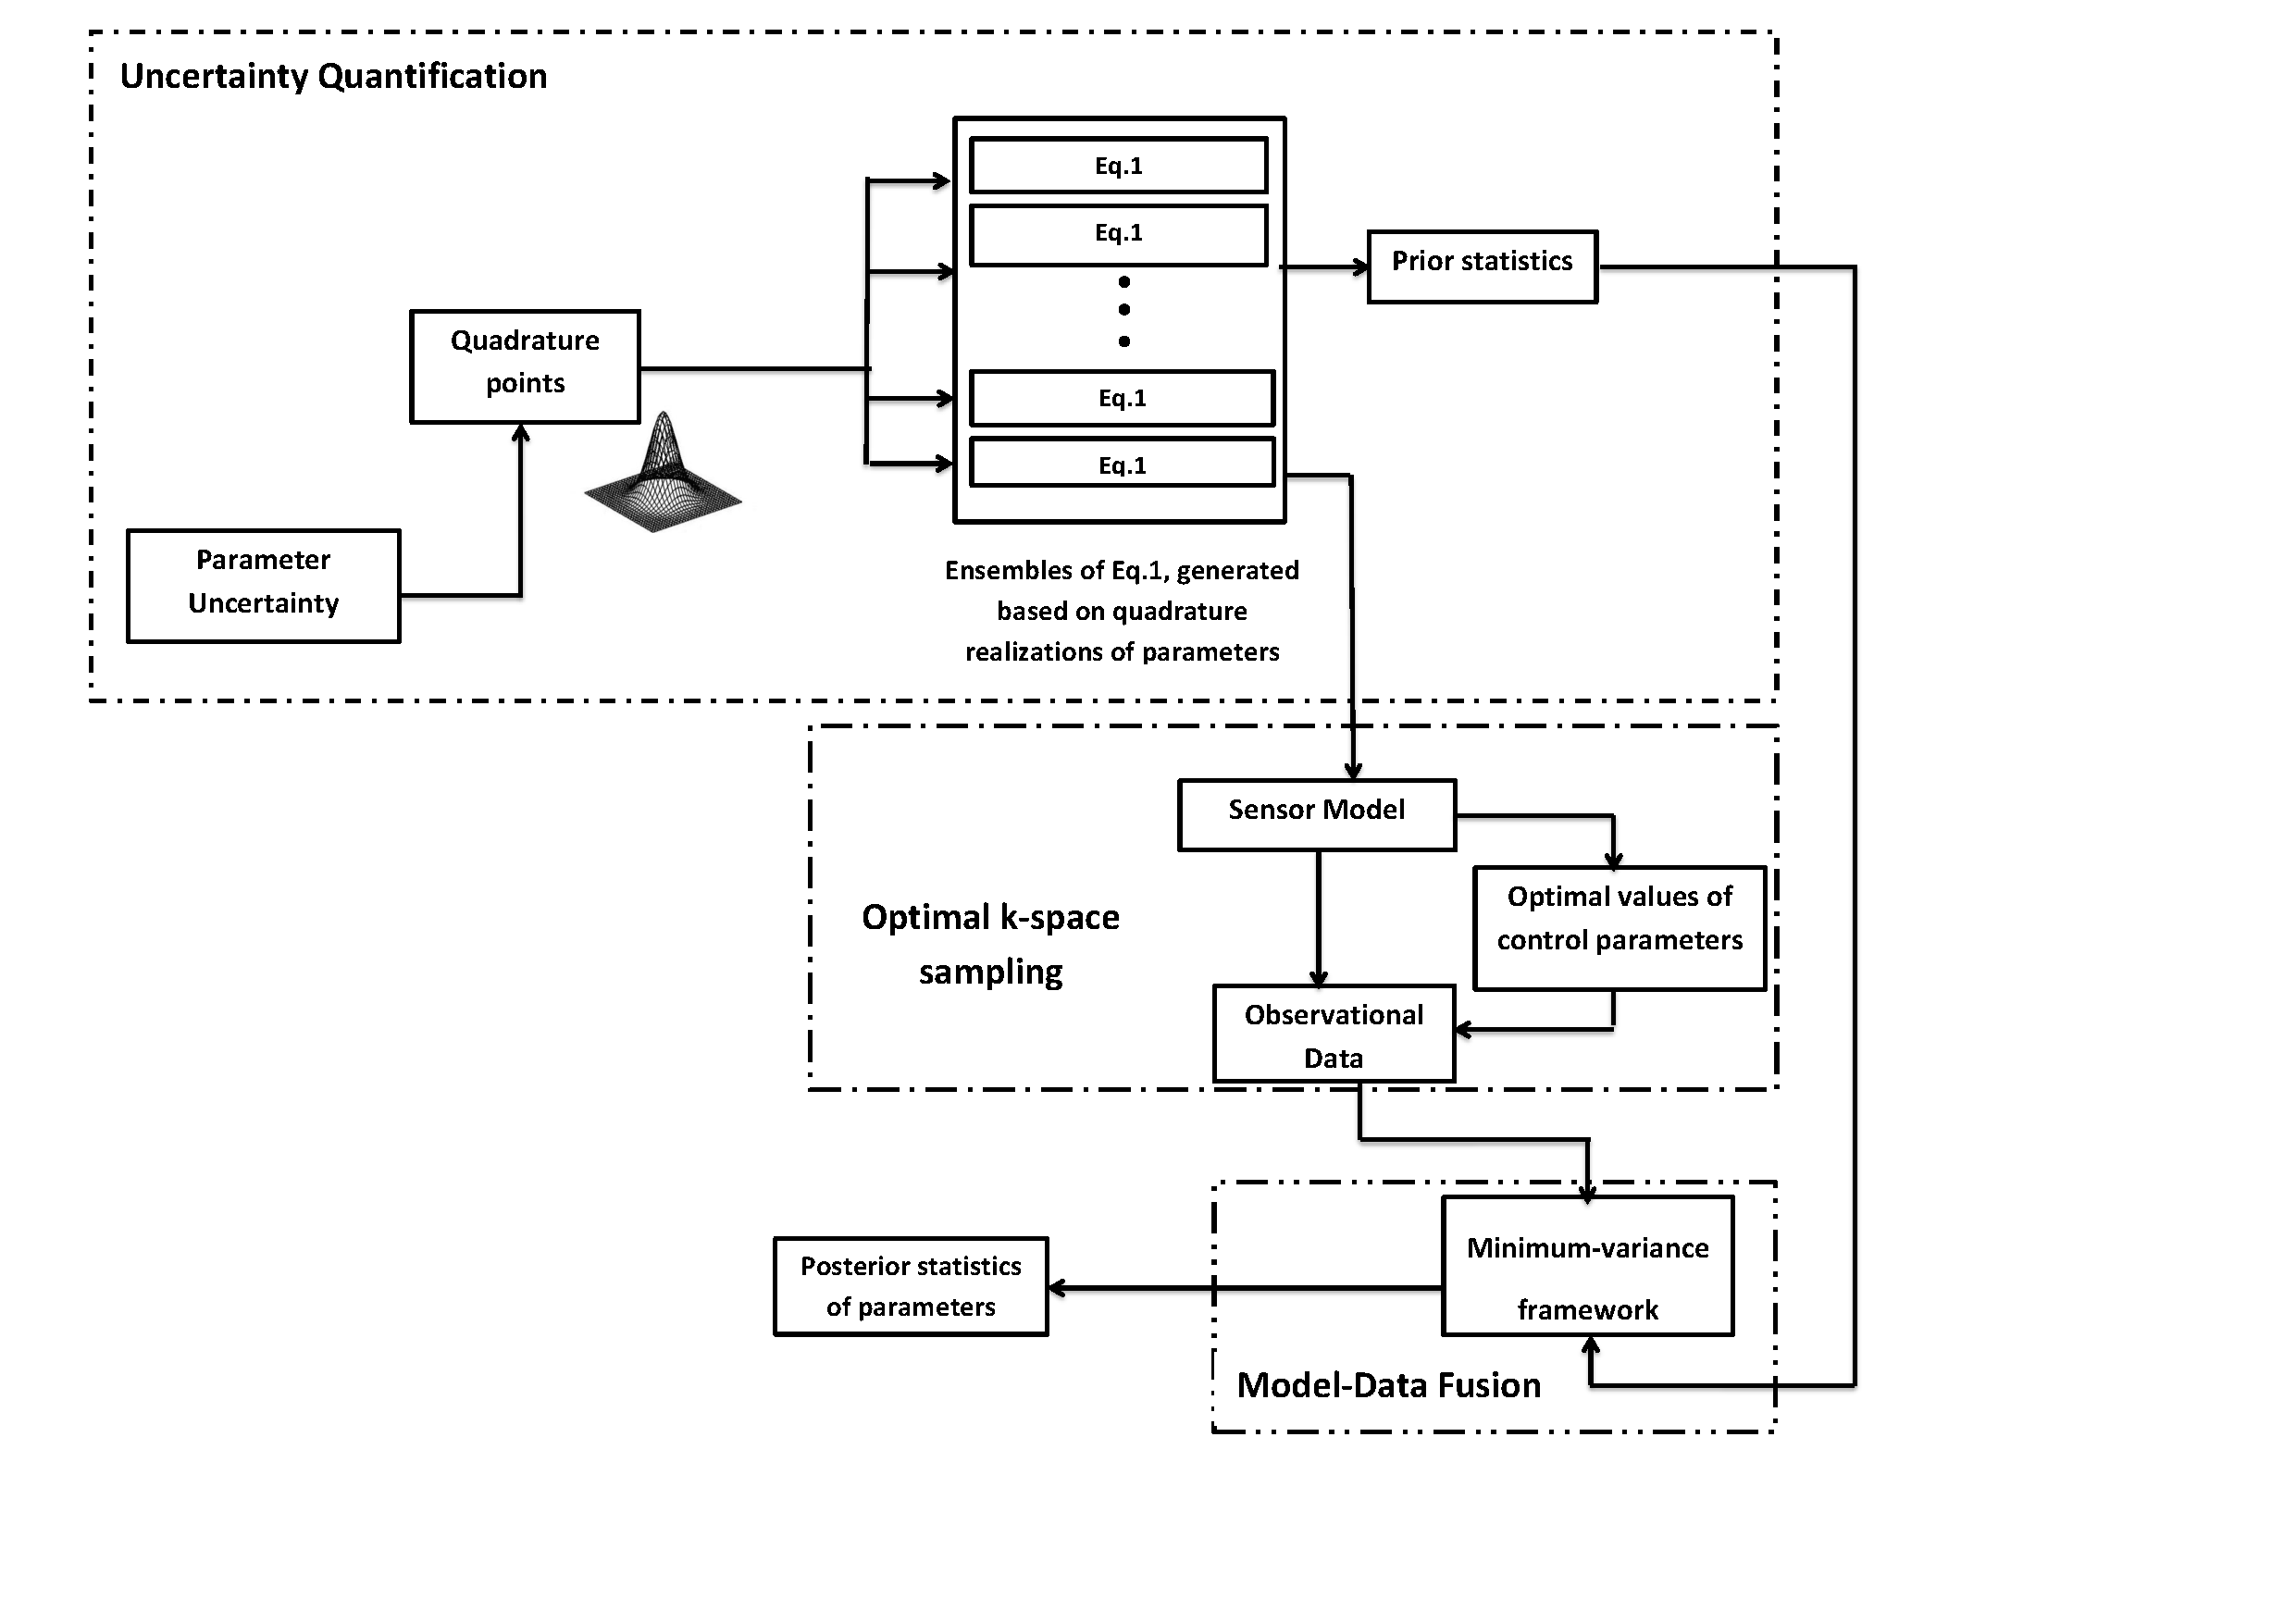
\includegraphics[trim = 1.5cm 3cm 8cm 0.5cm, clip,width=5in,height=4.5in]{flowchart.pdf}
\caption{Schematic view of the estimation process}
\end{figure}


%\begin{figure}[htb!]
%\begin{tabular}{ccc}
%\hspace{-0.25in}\subfigure{\includegraphics[width=2.5in]{pics/t2.eps}}&
%\hspace{-0.25in}\subfigure{\includegraphics[width=2.5in]{pics/t2meas.eps}}&
%\hspace{-0.25in}\subfigure{\includegraphics[width=2.5in]{pics/err2.eps}}
%\end{tabular}
%\caption{Temperature map over slice 2 a) Reconstructed temperature, b) observed temperature, c) the error between the reconstruction and measurement.}\label{t2}
%\end{figure}
% % t2 Fig
 

%\section*{Conclusion}
%In this manuscript, we provided new mathematical formulations to address the problem of parameter estimation in presence of large number of data observations. The key point of these formulations is to make use of Bayesian Central Limit Theorem, which approximates posterior distribution of parameter of interest with a Gaussian distribution, whose mean and covariance are provided using maximum likelihood estimate of the parameter and Fisher information, respectively. 
%
%It should be noted here that the only possible challenge in using these formulations is to evaluate the Fisher information. As we discussed before, finding Fisher information can be challenging in general, depending on the nonlinearities involved in observation operator $\mathcal{U}(\Teta)$.

%\bibliographystyle{IEEEtran}
%%\bibliographystyle{plain}
%\bibliography{refs}


\end{document}


